\documentclass[conference]{IEEEtran}
\IEEEoverridecommandlockouts

\usepackage[utf8]{inputenc}
\usepackage[T1]{fontenc}
\usepackage[brazil]{babel}
\usepackage{cite}
\usepackage{amsmath,amssymb,amsfonts}
\usepackage{algorithmic}
\usepackage{graphicx}
\usepackage{textcomp}
\usepackage{xcolor}
\usepackage{float}
\usepackage{multirow}
\usepackage{epstopdf}

\graphicspath{{figuras/}{./}}

\def\BibTeX{{\rm B\kern-.05em{\sc i\kern-.025em b}\kern-.08em
    T\kern-.1667em\lower.7ex\hbox{E}\kern-.125emX}}

\title{Sensibilidade por Camada e Fusão Adaptativa com Mistura de
Especialistas em Modelos Profundos para Classificação de Cor e Textura%
\thanks{Este trabalho foi apoiado pelo Conselho Nacional de
        Desenvolvimento Cient\'{i}fico e Tecnol\'{o}gico (CNPq, Brasil).}}

\author{
    \IEEEauthorblockN{
        Arlete T. Beuren\textsuperscript{1},
        Thiago Naves\textsuperscript{1},
        Leonardo J. R. Pinto\textsuperscript{1},
        Jonathan de Matos\textsuperscript{2},
        Alceu S. Britto Jr.\textsuperscript{2,3}
    }
    \IEEEauthorblockA{
        \textsuperscript{1}Universidade Tecnol\'{o}gica Federal do Paran\'{a} (UTFPR), Santa Helena (PR), Brasil\\
        E-mail: arletebeuren@utfpr.edu.br
        \\
        \textsuperscript{2}Universidade Estadual de Ponta Grossa (UEPG), Ponta Grossa (PR), Brasil\\
        E-mail: jonathan@uepg.br
        \\
        \textsuperscript{3}Pontif\'{i}cia Universidade Cat\'{o}lica do Paran\'{a} (PUCPR), Brasil\\
        E-mail: alceu@ppgia.pucpr.br
    }
}

\begin{document}

\maketitle

% -----------------------------------------------------------------------
\begin{abstract}

Este estudo aborda o desafio de extrair efetivamente o conte\'{u}do de
imagens com base em atributos visuais espec\'{i}ficos --- cor, textura ou
sua combina\c{c}\~{a}o --- e prop\~{o}e uma estrat\'{e}gia de fus\~{a}o
adaptativa baseada em Mistura de Especialistas~(MoE).
Experimentos s\~{a}o conduzidos com cinco arquiteturas --- ResNet-50,
VGG-16, iBOT, VMamba e LMFCN --- em um conjunto de dados de moda com
1.000 imagens de cor e 1.000 imagens de textura.
O \emph{Experimento~1} confirma que camadas iniciais s\~{a}o mais
eficazes para classifica\c{c}\~{a}o de cor, enquanto camadas profundas
se destacam no reconhecimento de textura, padr\~{a}o que se generaliza
de CNNs cl\'{a}ssicas a Vision Transformers e Modelos de Espa\c{c}o de
Estado.
O \emph{Experimento~2} mostra que a concatena\c{c}\~{a}o simples de
caracter\'{i}sticas de camadas iniciais e profundas geralmente n\~{a}o
supera representa\c{c}\~{o}es especializadas de camada \'{u}nica.
O \emph{Experimento~3} introduz um modelo MoE trein\'{a}vel que, por
meio de um roteador aprendido, pondera adaptativamente as contribui\c{c}\~{o}es
das camadas inicial (sens\'{i}vel a cor) e profunda (sens\'{i}vel a
textura) por imagem.
O MoE supera o Experimento~1 e o Experimento~2 em quase todas as
arquiteturas, atingindo at\'{e} 98,13\% com VMamba em textura e 98,13\%
com iBOT em cor --- melhorias de 3,80 e 2,27 pontos percentuais sobre as
melhores camadas individuais, respectivamente.

\end{abstract}

\begin{IEEEkeywords}
Redes Neurais Convolucionais, Modelos Profundos, Atributos Visuais,
Vision Transformers, Modelos de Espa\c{c}o de Estado, Mistura de
Especialistas, Recupera\c{c}\~{a}o de Imagens.
\end{IEEEkeywords}

% -----------------------------------------------------------------------
\section{Introdu\c{c}\~{a}o}

A Recupera\c{c}\~{a}o de Imagens Baseada em Conte\'{u}do (CBIR) tem
amplas aplica\c{c}\~{o}es em com\'{e}rcio eletr\^{o}nico, imagens
m\'{e}dicas e vigil\^{a}ncia~\cite{b1,b12}.
Um desafio central \'{e} extrair atributos visuais relevantes --- cor,
textura ou sua combina\c{c}\~{a}o --- para corresponder a consultas de
usu\'{a}rios (Figura~\ref{fig_patterns}).

\begin{figure}[htbp]
\centerline{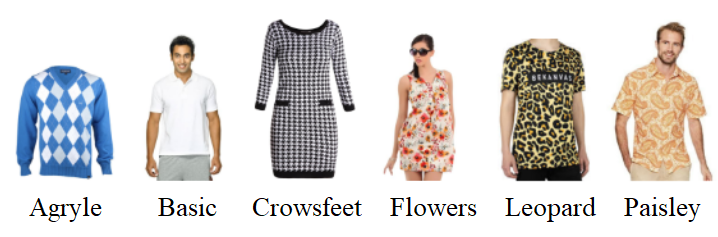
\includegraphics[width=0.48\textwidth]{fig_texture_samples.png}}
\caption{Seis padr\~{o}es distintos baseados em cor e textura
         (adaptado de~\cite{b2}).}
\label{fig_patterns}
\end{figure}

A extra\c{c}\~{a}o de caracter\'{i}sticas de cor e textura \'{e} t\'{o}pico
central em CBIR.
Descritores cl\'{a}ssicos de cor incluem histogramas e momentos de cor,
que capturam propriedades estat\'{i}sticas das distribui\c{c}\~{o}es
cromáticas~\cite{b24}.
Para textura, filtros de Gabor e Padr\~{o}es Bin\'{a}rios Locais (LBP)
s\~{a}o amplamente utilizados~\cite{b25}.

Com o advento do aprendizado profundo, Baloian et al.~\cite{b2}
demonstraram que diferentes camadas de CNN exibem sensibilidade
espec\'{i}fica a atributos, com camadas iniciais respondendo mais a
informa\c{c}\~{o}es de cor e camadas profundas capturando padr\~{o}es de
textura.
Contudo, o comportamento de representa\c{c}\~{o}es por atributo em
arquiteturas modernas --- Vision Transformers e Modelos de Espa\c{c}o de
Estado --- permanece pouco explorado, e estrat\'{e}gias de fus\~{a}o
adaptativa entre camadas especializadas s\~{a}o ainda escassas.

Neste trabalho, avaliamos e comparamos arquiteturas cl\'{a}ssicas e
modernas para classifica\c{c}\~{a}o baseada em cor e textura.
Como principal contribui\c{c}\~{a}o, propomos um modelo de fus\~{a}o
adaptativa baseado em Mistura de Especialistas~(MoE) que aprende, por
imagem, os pesos relativos das camadas inicial (cor) e profunda (textura)
por meio de um roteador trein\'{a}vel.

O conjunto de dados~\cite{b2} consiste em imagens de moda divididas em
um \textbf{subconjunto de cor} (1.000 imagens, 10 classes de cor) e um
\textbf{subconjunto de textura} (1.000 imagens, 10 classes de padr\~{a}o
de textura).

As principais contribui\c{c}\~{o}es deste trabalho s\~{a}o:
\begin{itemize}
  \item An\'{a}lise abrangente de sensibilidade por camada em CNNs
        cl\'{a}ssicas, Vision Transformers e Modelos de Espa\c{c}o de
        Estado;
  \item Benchmark comparativo de VGG-16, ResNet-50, iBOT, VMamba e LMFCN
        para classifica\c{c}\~{a}o por cor e textura;
  \item Demonstra\c{c}\~{a}o experimental de que fus\~{a}o por
        concatena\c{c}\~{a}o simples n\~{a}o melhora o desempenho em
        tarefas espec\'{i}ficas de atributos;
  \item Proposta e avalia\c{c}\~{a}o de modelo MoE para fus\~{a}o
        adaptativa de camadas, superando concatena\c{c}\~{a}o e
        representa\c{c}\~{o}es de camada \'{u}nica na maioria dos
        cen\'{a}rios.
\end{itemize}

% -----------------------------------------------------------------------
\section{Trabalhos Relacionados}

O uso de redes neurais convolucionais para representar similaridade entre
objetos tem sido amplamente explorado.
Baloian et al.~\cite{b2} investigaram o comportamento das camadas do
ResNet-50 para recupera\c{c}\~{a}o por cor e textura, mostrando que
camadas convolucionais iniciais s\~{a}o mais sens\'{i}veis \`{a} cor e
camadas profundas capturam melhor padr\~{o}es de textura.
Caracter\'{i}sticas foram extra\'{i}das com GAP em cada bloco residual e
avaliadas com kNN em 5 repeti\c{c}\~{o}es de holdout 70/30~\cite{b3}.

Zeiler e Fergus~\cite{bzeiler} mostraram que camadas iniciais de CNN
codificam bordas e cores, enquanto camadas profundas capturam padr\~{o}es
estruturais; Kazami et al.~\cite{bkazami} reportaram comportamento
an\'{a}logo em ViTs.
Ao contr\'{a}rio desses estudos qualitativos, este trabalho realiza uma
avalia\c{c}\~{a}o quantitativa sistem\'{a}tica em CNNs, ViTs e SSMs, e
prop\~{o}e fus\~{a}o adaptativa trein\'{a}vel fundamentada nesses
resultados.

Aprendizado de representa\c{c}\~{a}o para reconhecimento de atributos
foi explorado via redes neurais~\cite{b10,b11} e arquiteturas
Siamesas~\cite{b8}.
Descritores cl\'{a}ssicos de CBIR incluem caracter\'{i}sticas de textura
baseadas em wavelets~\cite{b13} e matrizes de co-ocorr\^{e}ncia de
cor~\cite{b15}.
Estrat\'{e}gias de fus\~{a}o multicamada --- concatena\c{c}\~{a}o, fus\~{a}o
tardia e combina\c{c}\~{a}o baseada em aten\c{c}\~{a}o~\cite{b26,b27} ---
foram propostas, mas sua efetividade para tarefas espec\'{i}ficas de
atributos permanece limitada.

Arquiteturas recentes incluem Mamba/VMamba~\cite{b16} (SSM, tempo linear),
iBOT~\cite{b17} (ViT autossupervisionado) e LMFCN~\cite{b28} (FCN com
SVM de grande margem).
MoE~\cite{bmoe_orig} utiliza um roteador para ponderar especialistas
locais; Cao et al.~\cite{bmoe_cao} o aplicaram a fus\~{a}o multimodal.
Seu uso para sele\c{c}\~{a}o de camadas por profundidade em um \'{u}nico
backbone permanece inexplorado --- a lacuna que este trabalho aborda.

% -----------------------------------------------------------------------
\section{Modelos de Backbone Avaliados}

Esta se\c{c}\~{a}o descreve as cinco arquiteturas de backbone utilizadas
nos experimentos. A Tabela~\ref{tab_backbones} resume suas propriedades
principais e a configura\c{c}\~{a}o de camadas usada no modelo MoE.

\begin{table}[htbp]
\caption{Resumo das arquiteturas de backbone avaliadas e configura\c{c}\~{a}o
         das camadas no MoE (E = inicial, P = profunda).}
\begin{center}
\begin{tabular}{c|c|c|c|c}
\hline
\textbf{Backbone} & \textbf{Tipo} & \textbf{Extr.} & \textbf{Dims} & \textbf{MoE E/P} \\
\hline
VGG-16    & CNN   & GAP/bloco  & 64--512   & Bl.1/Bl.3  \\
ResNet-50 & CNN   & GAP/res.blk& 256--2048 & RB1/RB3    \\
iBOT      & ViT   & token CLS  & 384       & Bl.2/Bl.9  \\
VMamba    & SSM   & GAP/est\'{a}gio  & 96--768   & Es.1/Es.2  \\
LMFCN     & FCN+SVM & camada SVM& 640--2560 & --         \\
\hline
\end{tabular}
\label{tab_backbones}
\end{center}
\end{table}

\subsection{ResNet-50}

ResNet-50~\cite{b4} \'{e} uma CNN de 50 camadas com conex\~{o}es
residuais baseadas em identidade.
Caracter\'{i}sticas s\~{a}o extra\'{i}das de cada bloco residual via GAP.

\subsection{VGG-16}

VGG-16~\cite{b7} empilha camadas convolucionais $3{\times}3$ em 5 blocos.
Caracter\'{i}sticas s\~{a}o extra\'{i}das via GAP em cada bloco.

\subsection{VMamba}

VMamba~\cite{b16} \'{e} um Modelo de Espa\c{c}o de Estado Estruturado
(SSM) que processa sequ\^{e}ncias em tempo linear por varredura seletiva.
Utilizamos a variante VMamba-Tiny com caracter\'{i}sticas extra\'{i}das
via GAP em cada est\'{a}gio.

\subsection{iBOT}

iBOT~\cite{b17} \'{e} um framework ViT autossupervisionado com
modelagem mascarada de imagens e tokenizador \textit{online}
(ViT-S/16, 12 blocos, token CLS).

\subsection{LMFCN}

LMFCN~\cite{b28} treina FCNs otimizadas para classifica\c{c}\~{a}o SVM
de grande margem.
Avaliamos variantes TCNN (3--6 camadas) e ResNet-18.
Devido ao acoplamento SVM--FCN, o LMFCN \'{e} avaliado apenas nos
Experimentos~1 e~2.

% -----------------------------------------------------------------------
\section{Metodologia Experimental}

\subsection{Base de Dados e Protocolo}

O conjunto de dados~\cite{b2} consiste em 10 classes de cor e 10 classes
de textura com 100 imagens por classe, totalizando 1.000 imagens por
tarefa.
Os dados foram divididos em 70\% treino e 30\% teste em 5 repeti\c{c}\~{o}es
de holdout estratificado.
Os vetores de caracter\'{i}sticas s\~{a}o avaliados com classificador
k-vizinhos mais pr\'{o}ximos (kNN, $k=5$, dist\^{a}ncia euclidiana).
Na avalia\c{c}\~{a}o de recupera\c{c}\~{a}o, o conjunto de treino serve
como gal\^{e}ria, garantindo conjuntos de consulta e base disjuntos.

\subsection{An\'{a}lise de Sensibilidade por Camada}

Para cada arquitetura, caracter\'{i}sticas s\~{a}o extra\'{i}das de cada
camada ou bloco individualmente.
CNNs usam GAP para produzir um vetor por camada; iBOT usa o token CLS;
VMamba aplica GAP ao mapa de caracter\'{i}sticas de cada est\'{a}gio.
Para o LMFCN, avaliamos variantes TCNN (3--6 camadas) e ResNet-18 com 2
ou 4 blocos residuais.

\subsection{Fus\~{a}o por Concatena\c{c}\~{a}o Inicial--Profunda}

Para cada backbone, as caracter\'{i}sticas da melhor camada de cor~(E) e
da melhor camada de textura~(P) s\~{a}o concatenadas:
$z = [f_E \; ; \; f_P]$, e o vetor resultante \'{e} avaliado com kNN.

\subsection{Fus\~{a}o Adaptativa com Mistura de Especialistas}

O modelo MoE proposto aprende, por imagem, pesos adaptativos $\alpha$ e
$\beta$ para as camadas inicial e profunda, respectivamente.

\textbf{Arquitetura.} Para cada backbone, duas cabe\c{c}as de proje\c{c}\~{a}o
$h_E$ e $h_P$ --- compostas por camada linear, LayerNorm e ReLU ---
mapeiam caracter\'{i}sticas de dimens\~{o}es heterog\^{e}neas para um
espa\c{c}o comum de dimens\~{a}o $d=256$.
Um Roteador (MLP de duas camadas com Softmax) recebe a concatena\c{c}\~{a}o
$[h_E(f_E) ; h_P(f_P)]$ e produz pesos $\alpha$ e $\beta$ com
$\alpha + \beta = 1$.
O embedding final \'{e}:
\begin{equation}
    z = \alpha \cdot h_E(f_E) + \beta \cdot h_P(f_P).
    \label{eq:moe}
\end{equation}

O backbone \'{e} congelado durante o treino; apenas $h_E$, $h_P$ e o
Roteador s\~{a}o atualizados.
Uma cabe\c{c}a linear auxiliar supervisiona o treino com perda de
entropia cruzada; na avalia\c{c}\~{a}o, apenas os embeddings $z$ s\~{a}o
usados com kNN.

\textbf{Protocolo de treino.}
Otimizador AdamW, $lr = 10^{-4}$, decaimento de peso $= 10^{-5}$,
CosineAnnealingLR com $T_{\max} = 30$ \'{e}pocas, lote de 32,
augmenta\c{c}\~{a}o b\'{a}sica (recorte aleat\'{o}rio $224{\times}224$
e espelhamento horizontal) apenas no treino.
Avalia\c{c}\~{a}o final: kNN com $k=5$ e StandardScaler nos embeddings
$z$, com o mesmo protocolo de 5 repeti\c{c}\~{o}es de holdout.

A Tabela~\ref{tab_moe_config} resume as sele\c{c}\~{o}es de camada por
backbone no modelo MoE.

\begin{table}[htbp]
\caption{Configura\c{c}\~{a}o das camadas inicial e profunda por backbone
         no modelo MoE.}
\begin{center}
\begin{tabular}{c|c|c|c|c}
\hline
\textbf{Backbone} & \textbf{Inicial (E)} & \textbf{Dim~E}
                  & \textbf{Profunda (P)} & \textbf{Dim~P} \\
\hline
VGG-16    & Bloco 1      & 64   & Bloco 3      & 256  \\
ResNet-50 & Bl. Res. 1   & 256  & Bl. Res. 3   & 1024 \\
iBOT      & Bloco 2      & 384  & Bloco 9      & 384  \\
VMamba    & Est\'{a}gio 1 & 192  & Est\'{a}gio 2 & 384  \\
\hline
\end{tabular}
\label{tab_moe_config}
\end{center}
\end{table}

% -----------------------------------------------------------------------
\section{Resultados Experimentais}

Os resultados cobrem sensibilidade por camada~(Se\c{c}\~{o}es~V-A e~V-B),
estrat\'{e}gias de fus\~{a}o~(V-C e~V-D) e avalia\c{c}\~{a}o CBIR com
mAP@10, R@1 e R@5~(V-E).

\subsection{Sensibilidade por Camada}

A Tabela~\ref{tab_best_layer} resume a melhor camada por backbone para
classifica\c{c}\~{a}o de cor e textura.
Em todas as arquiteturas, camadas iniciais consistentemente atingem maior
acur\'{a}cia de cor, enquanto camadas profundas s\~{a}o mais eficazes
para textura --- confirmando e estendendo o padr\~{a}o reportado para
ResNet-50 em~\cite{b2}.
No VGG-16, a Camada~1 atinge 95,13\% para cor e a Camada~4 atinge 94,73\%
para textura.
O ResNet-50 segue a mesma tend\^{e}ncia: Bloco Residual~2 para
cor~(95,87\%) e Bloco~3 para textura~(93,27\%).
O iBOT apresenta o gradiente mais acentuado entre seus 12 blocos ---
a acur\'{a}cia de cor cai de 94,53\% no Bloco~0 para 62,80\% no
Bloco~11, enquanto textura sobe para 97,20\% no Bloco~9, o maior valor
entre todas as arquiteturas avaliadas.
O VMamba exibe uma vers\~{a}o comprimida do mesmo padr\~{a}o, com
Est\'{a}gio~1 melhor para cor~(94,80\%) e Est\'{a}gio~2 para
textura~(94,33\%).

\begin{table}[htbp]
\caption{Melhor camada por backbone para classifica\c{c}\~{a}o de cor e
         textura (\%). Negrito: maior valor por coluna de atributo.}
\begin{center}
\begin{tabular}{c|c|c|c|c|c|c}
\hline
\textbf{Backbone} & \textbf{Mel. Cor} & \textbf{Cor} & \textbf{DP}
                  & \textbf{Mel. Tex.} & \textbf{Tex.} & \textbf{DP} \\
\hline
VGG-16    & Camada 1 & 95,13          & 0,81 & Camada 4 & 94,73          & 0,74 \\
ResNet-50 & BR 2     & \textbf{95,87} & 0,50 & BR 3     & 93,27          & 0,25 \\
iBOT      & Bloco 2  & \textbf{95,87} & 1,05 & Bloco 9  & \textbf{97,20} & 0,54 \\
VMamba    & Est. 1   & 94,80          & 0,62 & Est. 2   & 94,33          & 1,40 \\
\hline
\end{tabular}
\label{tab_best_layer}
\end{center}
\end{table}

A Figura~\ref{fig_depth} ilustra as curvas completas de desempenho por
profundidade, evidenciando o padr\~{a}o inverso entre cor e textura.

\begin{figure}[htbp]
\centerline{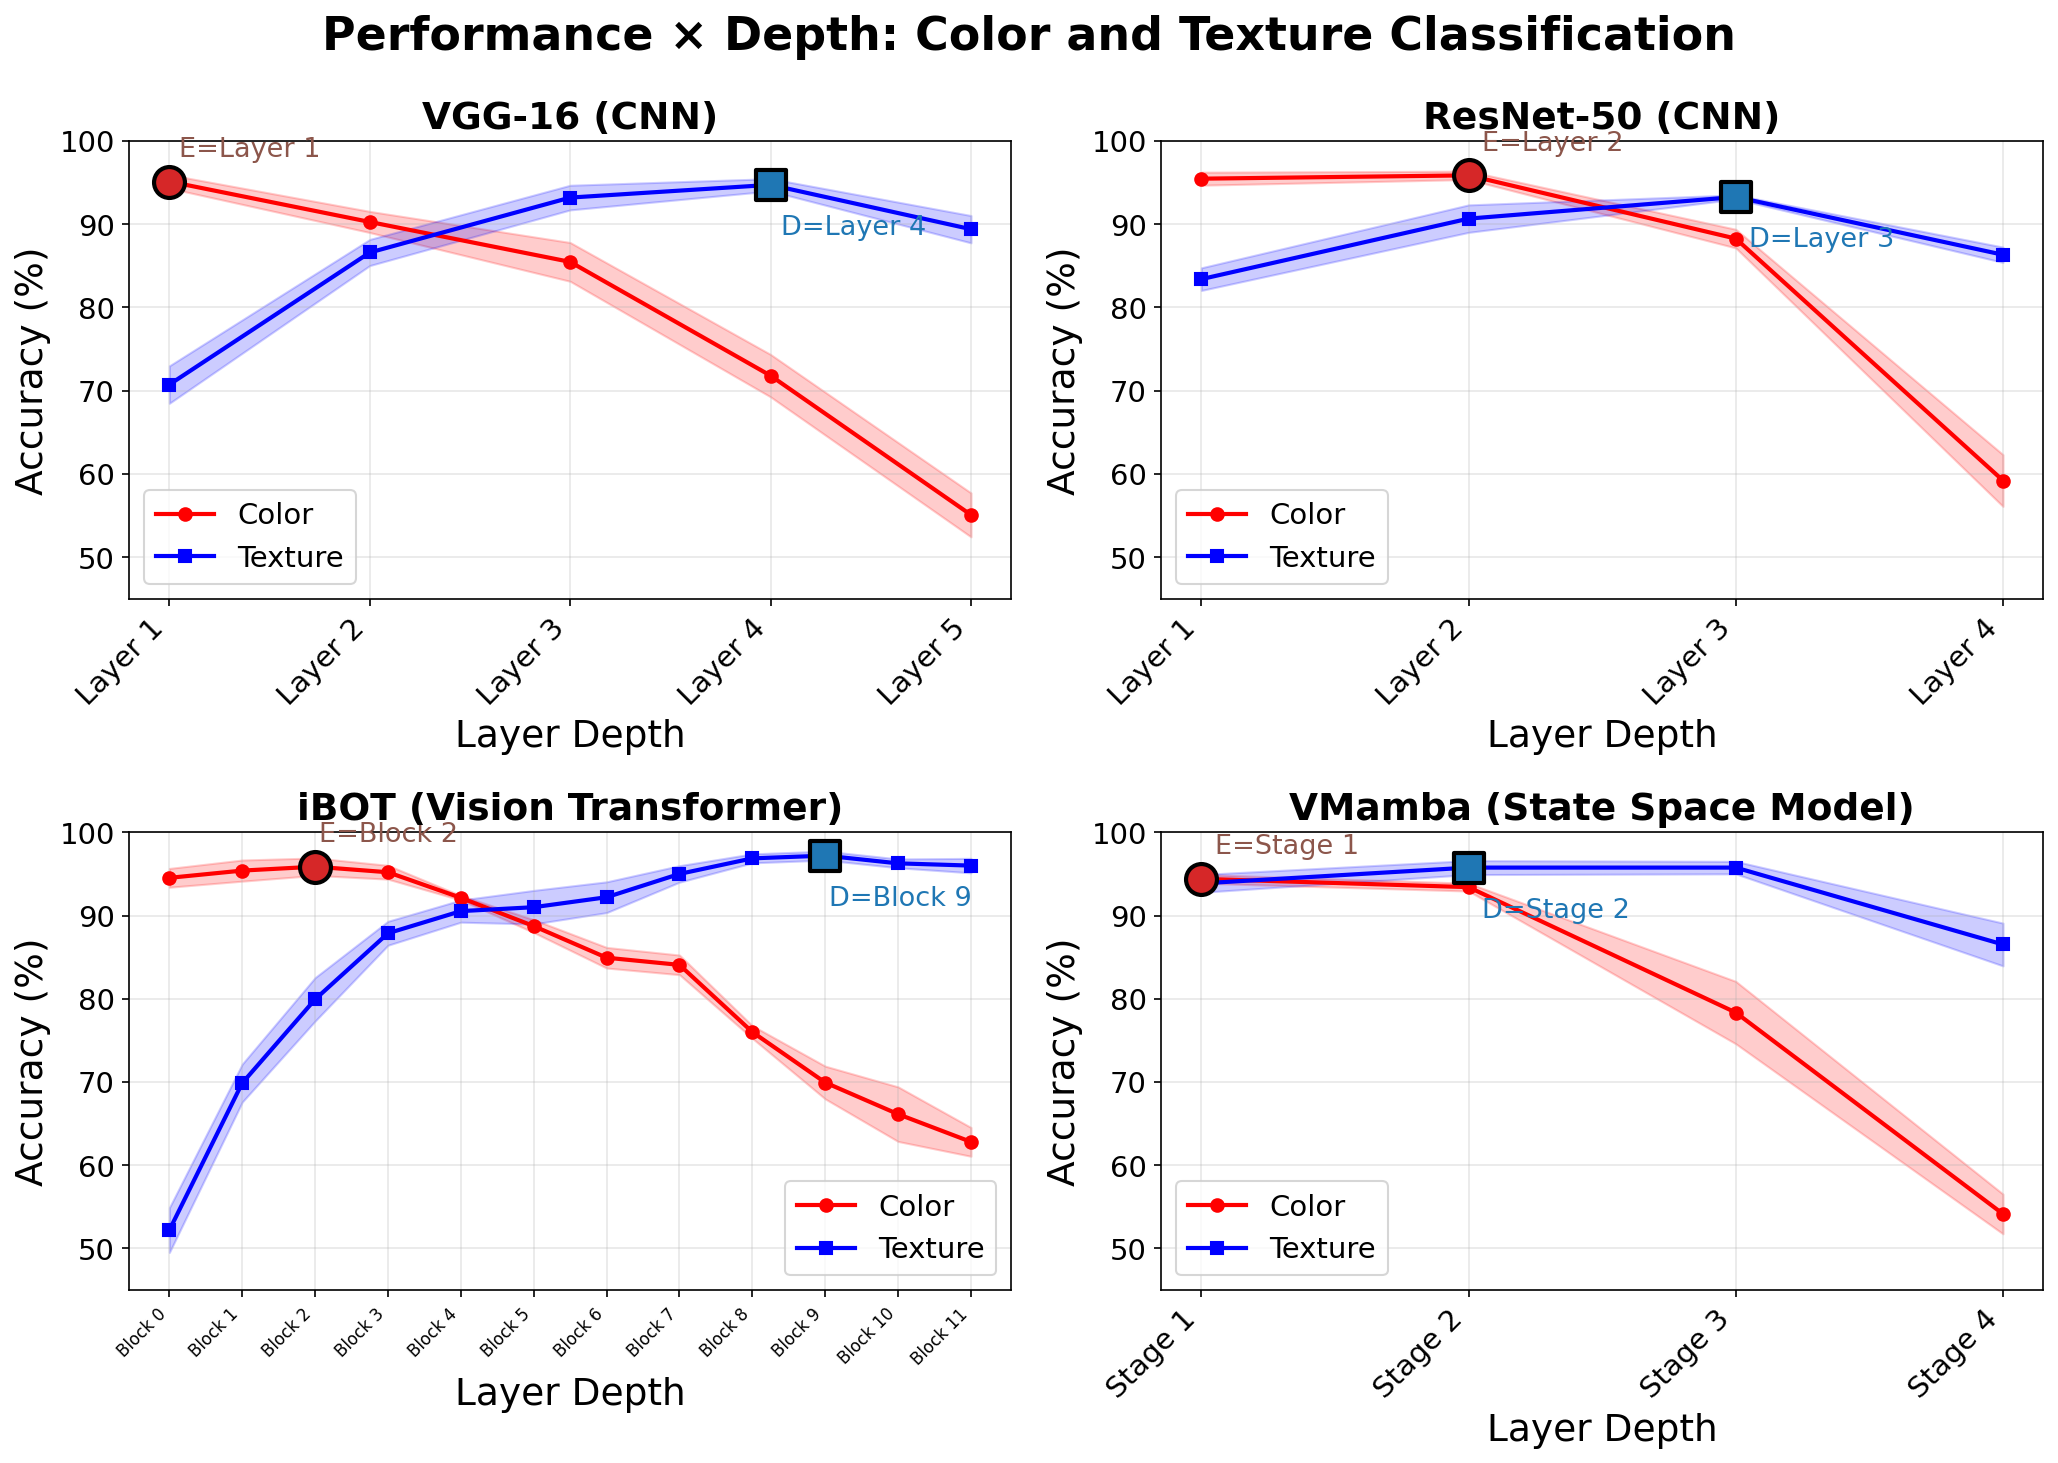
\includegraphics[width=0.48\textwidth]{curvas_desempenho_profundidade.png}}
\caption{Desempenho vs.\ profundidade: classifica\c{c}\~{a}o de cor e
         textura para VGG-16, ResNet-50, iBOT e VMamba. Marcadores
         indicam a melhor camada por atributo (E=cor, P=textura).}
\label{fig_depth}
\end{figure}

\subsection{Sensibilidade por Camada --- LMFCN}

A Tabela~\ref{tab1} apresenta os resultados do LMFCN.
No conjunto de textura, o aumento de profundidade do TCNN melhora
consistentemente o desempenho.
No conjunto de cor, maior acur\'{a}cia \'{e} obtida em camadas mais
iniciais.
O LMFCN com SVM atingiu 96,87\%$\pm$0,9 em textura (ResNet-18 com
2 blocos) e 97,73\%$\pm$0,95 em cor (TCNN3).

\begin{table}[htbp]
\caption{Acur\'{a}cia dos blocos convolucionais (CB) e residuais (BR) do
         ResNet-18 e das camadas TCNN usando LMFCN.}
\begin{center}
\begin{tabular}{c|c|c|c|c|c}
\hline
\textbf{M\'{e}todo} & \textbf{Cor} & \textbf{DP}
                    & \textbf{Tex.} & \textbf{DP} & \textbf{Dim} \\
\hline
TCNN3 Cam. 3      & \textbf{95,94} & 0,43 & \textbf{58,27} & 1,30 & 640  \\
TCNN4 Cam. 4      & \textbf{94,80} & 0,65 & \textbf{60,40} & 2,60 & 640  \\
TCNN5 Cam. 5      & 95,40 & 0,96 & \textbf{62,93} & 1,65 & 640  \\
TCNN6 Cam. 6      & 94,53 & 0,84 & \textbf{64,34} & 2,69 & 640  \\
ResNet-18(2) BR1  & \textbf{96,13} & 0,73 & 84,87 & 1,38 & 640  \\
ResNet-18(2) BR2  & 91,93 & 0,98 & \textbf{91,00} & 1,62 & 1280 \\
ResNet-18(4) BR1  & \textbf{95,93} & 0,98 & 84,13 & 1,59 & 640  \\
ResNet-18(4) BR3  & 89,53 & 1,37 & \textbf{92,47} & 1,48 & 2560 \\
\hline
\end{tabular}
\label{tab1}
\end{center}
\end{table}

\subsection{Resultados da Fus\~{a}o por Concatena\c{c}\~{a}o}

A Tabela~\ref{tab_concat} apresenta os resultados da fus\~{a}o por
concatena\c{c}\~{a}o para cor e textura, onde E denota a melhor camada
de cor, P a melhor camada de textura e Z a representa\c{c}\~{a}o fundida.

\begin{table}[htbp]
\caption{Resultados da fus\~{a}o por concatena\c{c}\~{a}o (\%). Negrito:
         melhor valor por linha.}
\begin{center}
\begin{tabular}{c|c|c|c|c|c}
\hline
\textbf{Backbone} & \textbf{Tarefa} & \textbf{E} & \textbf{P}
                  & \textbf{Z} & \textbf{$\Delta$} \\
\hline
\multirow{2}{*}{VGG-16}
  & Cor     & \textbf{95,13} & 71,80 & 86,13 & $-$9,00 \\
  & Textura & 70,73 & \textbf{94,73} & 94,73 & $+$0,00 \\
\hline
\multirow{2}{*}{ResNet-50}
  & Cor     & \textbf{95,87} & 88,27 & 94,13 & $-$1,73 \\
  & Textura & 90,67 & 93,27 & \textbf{93,53} & $+$0,27 \\
\hline
\multirow{2}{*}{iBOT}
  & Cor     & \textbf{95,87} & 69,93 & 74,33 & $-$21,53 \\
  & Textura & 79,93 & \textbf{97,20} & 97,00 & $-$0,20 \\
\hline
\multirow{2}{*}{VMamba}
  & Cor     & \textbf{94,80} & 93,93 & 94,13 & $-$0,67 \\
  & Textura & 88,40 & \textbf{94,33} & 93,40 & $-$0,93 \\
\hline
\end{tabular}
\label{tab_concat}
\end{center}
\end{table}

Os resultados mostram que a concatena\c{c}\~{a}o simples geralmente n\~{a}o
melhora o desempenho.
Para cor, a fus\~{a}o degradou consistentemente a acur\'{a}cia em rela\c{c}\~{a}o
\`{a} camada de cor isolada (E), com iBOT apresentando a maior
degrada\c{c}\~{a}o~($-$21,53\%).
Para textura, os resultados foram mistos, com melhoria m\'{i}nima para
ResNet-50~($+$0,27\%) e degrada\c{c}\~{o}es menores para iBOT~($-$0,20\%)
e VMamba~($-$0,93\%).

\subsection{Resultados da Fus\~{a}o MoE Adaptativa}

A Tabela~\ref{tab_moe} apresenta os resultados do modelo MoE proposto.
Comparado \`{a} extra\c{c}\~{a}o por camada \'{u}nica e \`{a} fus\~{a}o
por concatena\c{c}\~{a}o, o MoE supera ambos em quase todas as
combina\c{c}\~{o}es backbone--atributo.

\begin{table}[htbp]
\caption{Resultados do modelo MoE para classifica\c{c}\~{a}o de cor e
         textura.}
\begin{center}
\begin{tabular}{c|c|c|c|c}
\hline
\textbf{Backbone} & \textbf{MoE Cor (\%)} & \textbf{DP}
                  & \textbf{MoE Tex. (\%)} & \textbf{DP} \\
\hline
VGG-16    & 94,20 & 1,68 & \textbf{95,80} & 1,63 \\
ResNet-50 & 95,87 & 0,88 & \textbf{97,73} & 0,65 \\
iBOT      & \textbf{98,13} & 0,69 & 94,80 & 1,17 \\
VMamba    & 97,20 & 0,45 & \textbf{98,13} & 0,62 \\
\hline
\end{tabular}
\label{tab_moe}
\end{center}
\end{table}

A Tabela~\ref{tab_comparacao} consolida a compara\c{c}\~{a}o entre as
tr\^{e}s estrat\'{e}gias.

\begin{table}[htbp]
\caption{Compara\c{c}\~{a}o entre camada \'{u}nica (Exp.\,1),
         concatena\c{c}\~{a}o (Exp.\,2) e MoE (Exp.\,3). Valores em \%.
         $\Delta_1$: ganho sobre camada \'{u}nica; $\Delta_2$: ganho
         sobre concatena\c{c}\~{a}o.}
\begin{center}
\begin{tabular}{c|c|c|c|c|c|c}
\hline
\textbf{Config.} & \textbf{Exp.1} & \textbf{Exp.2}
                 & \textbf{MoE} & \textbf{$\Delta_1$}
                 & \textbf{$\Delta_2$} & \textbf{Melhor} \\
\hline
VGG Cor    & 95,13 & 86,13 & 94,20 & $-$0,93 & $+$8,07  & Exp.1 \\
VGG Tex.   & 94,73 & 94,73 & 95,80 & $+$1,07 & $+$1,07  & \textbf{MoE} \\
ResNet Cor & 95,87 & 94,13 & 95,87 & $+$0,00 & $+$1,73  & Exp.1 \\
ResNet Tex.& 93,27 & 93,53 & 97,73 & $+$4,47 & $+$4,20  & \textbf{MoE} \\
iBOT Cor   & 95,87 & 74,33 & 98,13 & $+$2,27 & $+$23,80 & \textbf{MoE} \\
iBOT Tex.  & 97,20 & 97,00 & 94,80 & $-$2,40 & $-$2,20  & Exp.1 \\
VMamba Cor & 94,80 & 94,13 & 97,20 & $+$2,40 & $+$3,07  & \textbf{MoE} \\
VMamba Tex.& 94,33 & 93,40 & 98,13 & $+$3,80 & $+$4,73  & \textbf{MoE} \\
\hline
\end{tabular}
\label{tab_comparacao}
\end{center}
\end{table}

O MoE \'{e} o melhor ou empata em 6 das 8 configura\c{c}\~{o}es avaliadas.
As duas exce\c{c}\~{o}es --- VGG-16 cor e iBOT textura --- correspondem
a casos em que uma \'{u}nica camada especializada j\'{a} atinge desempenho
muito alto (95,13\% e 97,20\%, respectivamente), deixando pouco espa\c{c}o
para melhoria.
O ganho do MoE sobre a concatena\c{c}\~{a}o \'{e} expressivo em 7 das 8
configura\c{c}\~{o}es, especialmente para iBOT cor~($+$23,80~pp) e VMamba
textura~($+$4,73~pp); a exce\c{c}\~{a}o \'{e} iBOT textura, onde a
concatena\c{c}\~{a}o j\'{a} preserva a capacidade discriminativa do
Bloco~9~(97,00\%).

\subsection{Avalia\c{c}\~{a}o CBIR: mAP@10, R@1 e R@5}

A Tabela~\ref{tab_cbir} reporta a avalia\c{c}\~{a}o de recupera\c{c}\~{a}o
sob protocolo CBIR padr\~{a}o: para cada consulta, todas as imagens de
treino s\~{a}o ordenadas por dist\^{a}ncia euclidiana e as m\'{e}tricas
s\~{a}o computadas sobre os $K\!=\!10$ vizinhos mais pr\'{o}ximos.

\begin{table}[htbp]
\caption{Avalia\c{c}\~{a}o CBIR --- Cor e Textura (\%). Melhor valor por
         backbone e tarefa em \textbf{negrito}.}
\begin{center}
\footnotesize
\begin{tabular}{c|c|l|c|c|c}
\hline
\textbf{BB} & \textbf{Tar.} & \textbf{M\'{e}todo}
            & \textbf{mAP} & \textbf{R@1} & \textbf{R@5} \\
\hline
\multirow{8}{*}{\rotatebox{90}{VGG-16}}
  & \multirow{4}{*}{Cor}
    & Inicial (E) & \textbf{94,47} & \textbf{95,47} & \textbf{99,13} \\
  & & Profunda (P)& 72,92 & 72,20 & 91,53 \\
  & & Concat.     & 83,89 & 86,53 & 96,73 \\
  & & MoE         & 93,71 & 94,93 & 98,07 \\
  \cline{2-6}
  & \multirow{4}{*}{Tex.}
    & Inicial (E) & 70,87 & 70,33 & 91,27 \\
  & & Profunda (P)& 94,78 & 96,20 & \textbf{99,47} \\
  & & Concat.     & 94,53 & 96,13 & 99,27 \\
  & & MoE         & \textbf{95,98} & \textbf{96,80} & 99,07 \\
\hline
\multirow{8}{*}{\rotatebox{90}{ResNet-50}}
  & \multirow{4}{*}{Cor}
    & Inicial (E) & 94,51 & 96,13 & 99,00 \\
  & & Profunda (P)& 86,25 & 87,67 & 97,20 \\
  & & Concat.     & 92,40 & 93,93 & 98,33 \\
  & & MoE         & \textbf{96,09} & \textbf{96,07} & \textbf{98,67} \\
  \cline{2-6}
  & \multirow{4}{*}{Tex.}
    & Inicial (E) & 90,35 & 90,80 & 99,07 \\
  & & Profunda (P)& 93,72 & 95,60 & 99,20 \\
  & & Concat.     & 93,05 & 94,47 & 98,87 \\
  & & MoE         & \textbf{97,88} & \textbf{98,13} & \textbf{99,20} \\
\hline
\multirow{8}{*}{\rotatebox{90}{iBOT}}
  & \multirow{4}{*}{Cor}
    & Inicial (E) & 94,93 & 95,40 & 99,13 \\
  & & Profunda (P)& 71,85 & 72,00 & 92,47 \\
  & & Concat.     & 75,06 & 76,67 & 94,13 \\
  & & MoE         & \textbf{97,96} & \textbf{98,27} & \textbf{99,47} \\
  \cline{2-6}
  & \multirow{4}{*}{Tex.}
    & Inicial (E) & 78,90 & 79,33 & 94,33 \\
  & & Profunda (P)& \textbf{96,40} & \textbf{97,73} & \textbf{99,80} \\
  & & Concat.     & 96,30 & 97,67 & 99,73 \\
  & & MoE         & 95,10 & 95,40 & 98,53 \\
\hline
\multirow{8}{*}{\rotatebox{90}{VMamba}}
  & \multirow{4}{*}{Cor}
    & Inicial (E) & 93,20 & 94,33 & 98,47 \\
  & & Profunda (P)& 91,73 & 93,13 & 98,33 \\
  & & Concat.     & 92,51 & 93,67 & 98,40 \\
  & & MoE         & \textbf{96,91} & \textbf{96,87} & \textbf{99,07} \\
  \cline{2-6}
  & \multirow{4}{*}{Tex.}
    & Inicial (E) & 87,66 & 88,80 & 97,33 \\
  & & Profunda (P)& 93,52 & 95,53 & 99,13 \\
  & & Concat.     & 93,05 & 95,07 & 99,13 \\
  & & MoE         & \textbf{97,89} & \textbf{98,27} & \textbf{99,33} \\
\hline
\end{tabular}
\label{tab_cbir}
\end{center}
\end{table}

O MoE obteve as melhores m\'{e}tricas CBIR em 3 dos 4 backbones para cor
e 3 dos 4 para textura.
A exce\c{c}\~{a}o para iBOT textura espelha o resultado de acur\'{a}cia:
o Bloco~9 j\'{a} produz representa\c{c}\~{o}es t\~{a}o discriminativas
(mAP@10 = 96,40\%) que o roteador n\~{a}o consegue melhor\'{a}-las.
O ganho do MoE sobre a concatena\c{c}\~{a}o \'{e} especialmente expressivo
para iBOT cor~($+$22,90~pp em mAP@10).

\subsection{An\'{a}lise Qualitativa de Recupera\c{c}\~{a}o}

As Figuras~\ref{fig_retrieval_color} e~\ref{fig_retrieval_texture} mostram
exemplos representativos de recupera\c{c}\~{a}o com o backbone iBOT.
Cada linha exibe uma imagem de consulta (extremo esquerdo, borda cinza) e
seus 5 vizinhos mais pr\'{o}ximos por dist\^{a}ncia euclidiana; bordas
verdes indicam a classe correta e bordas vermelhas indicam erros.

\begin{figure}[htbp]
\centerline{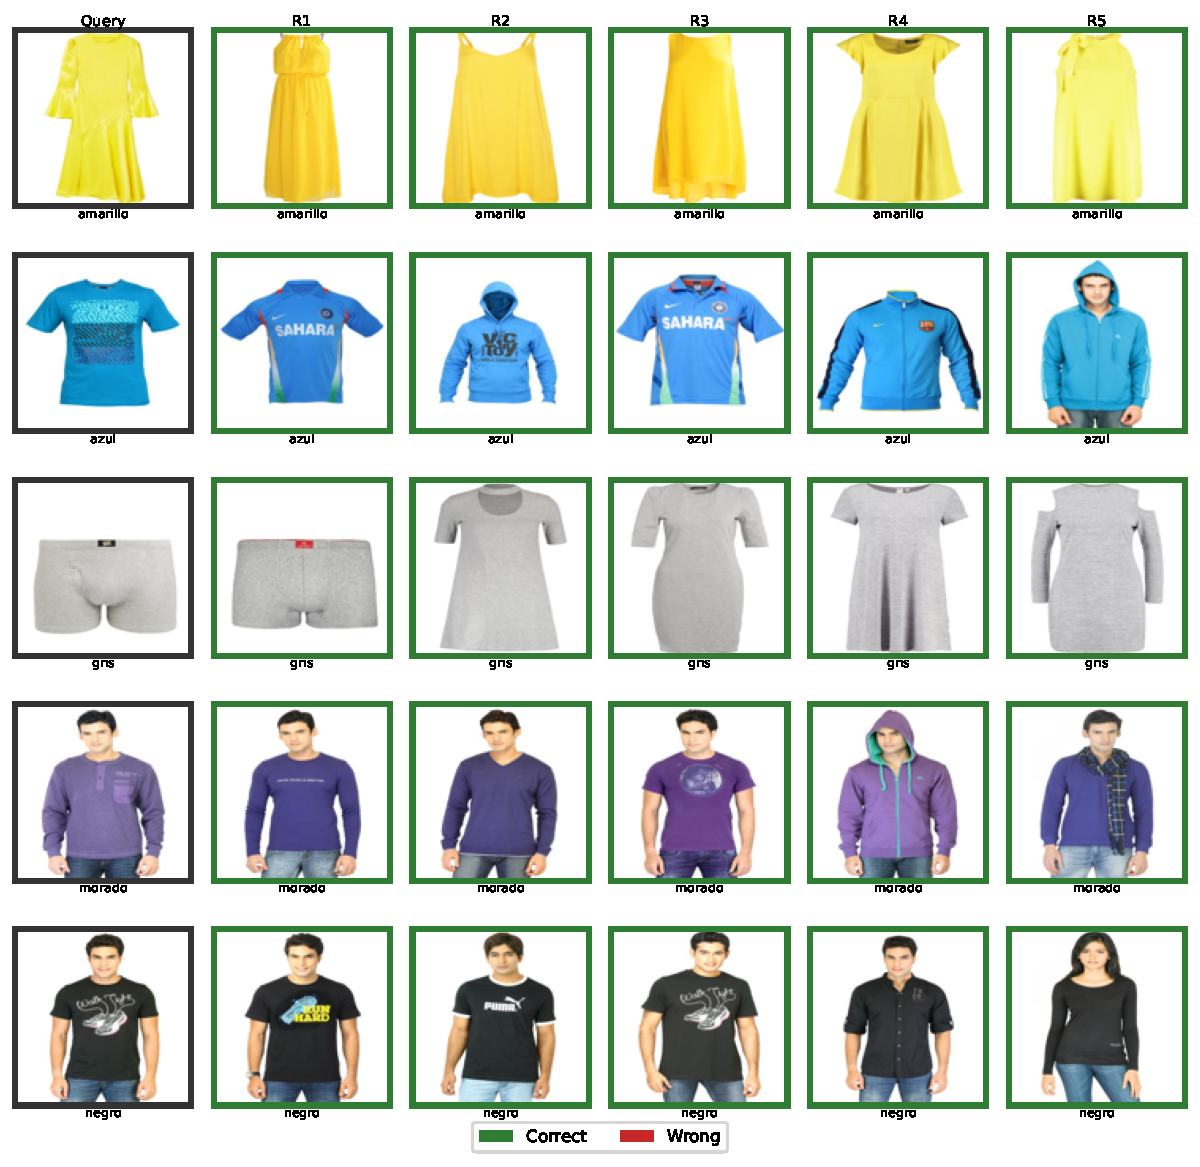
\includegraphics[width=0.48\textwidth]{fig_retrieval_color.pdf}}
\caption{Exemplos de recupera\c{c}\~{a}o top-5 para cor (iBOT Bloco~2,
         fold~1). Consultas: amarelo, azul, cinza, roxo, preto.
         Verde = classe correta; vermelho = erro.}
\label{fig_retrieval_color}
\end{figure}

Na recupera\c{c}\~{a}o por cor (Bloco~2), o modelo retorna
consistentemente pe\c{c}as da mesma cor independentemente do tipo de
roupa.
A coer\^{e}ncia visual reflete o alto mAP@10~(94,93\%) obtido nessa
camada.

\begin{figure}[htbp]
\centerline{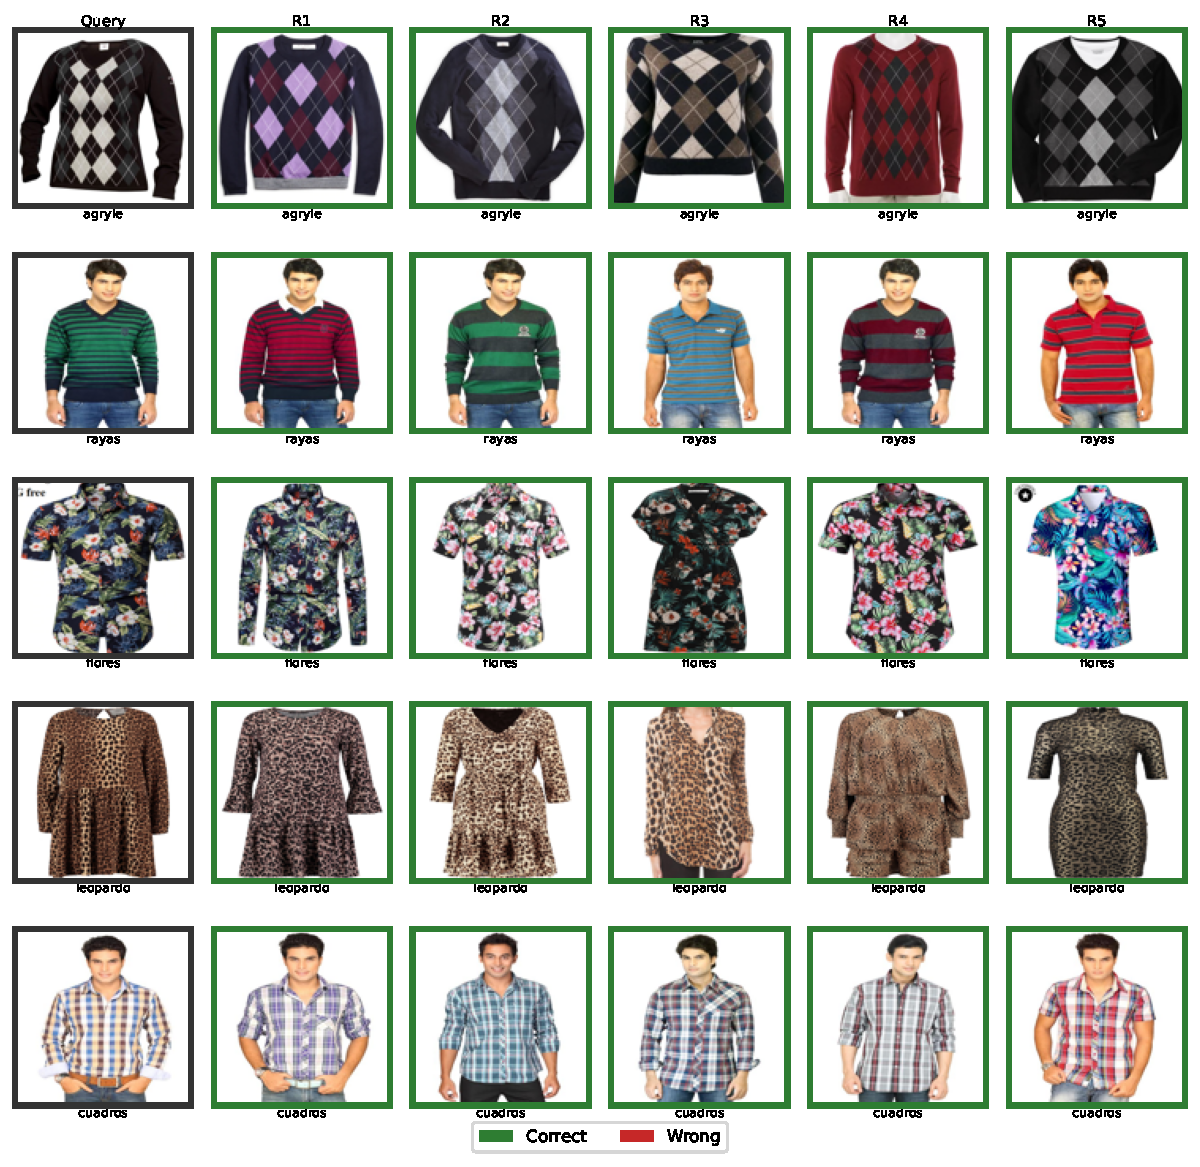
\includegraphics[width=0.48\textwidth]{fig_retrieval_texture.pdf}}
\caption{Exemplos de recupera\c{c}\~{a}o top-5 para textura (iBOT
         Bloco~9, fold~1). Consultas: argyle, listrado, floral, leopardo,
         xadrez. Verde = classe correta; vermelho = erro.}
\label{fig_retrieval_texture}
\end{figure}

Na recupera\c{c}\~{a}o por textura (Bloco~9), as representa\c{c}\~{o}es
do transformer profundo agrupam com \^{e}xito padr\~{o}es estruturais.
Os poucos erros envolvem padr\~{o}es visualmente amb\'{i}guos
(ex.: listras densas confundidas com xadrez), os mesmos observados na
m\'{e}trica mAP@10~(96,40\% no Bloco~9).

% -----------------------------------------------------------------------
\section{Discuss\~{a}o}

O padr\~{a}o de sensibilidade por camada --- camadas iniciais para cor,
camadas profundas para textura --- estende-se de CNNs
cl\'{a}ssicas~\cite{bzeiler} a ViTs~\cite{bkazami} e, como demonstrado
aqui, ao VMamba (SSM).
A acur\'{a}cia excepcional do iBOT em textura~(97,20\%) indica que o
objetivo de modelagem mascarada autossupervisionada favorece
representa\c{c}\~{o}es estruturais ricas; a dimensionalidade uniforme de
384d nos blocos do iBOT sugere que a qualidade da representa\c{c}\~{a}o,
e n\~{a}o seu tamanho, \'{e} o fator determinante.

O Experimento~2 demonstrou que a concatena\c{c}\~{a}o simples n\~{a}o
\'{e} uma estrat\'{e}gia eficaz para tarefas espec\'{i}ficas de atributos.
O modelo MoE~(Experimento~3) resolve essa limita\c{c}\~{a}o ao aprender
dinamicamente os pesos de contribui\c{c}\~{a}o por imagem.
O roteador trein\'{a}vel adapta-se ao conte\'{u}do: imagens mais
discriminativas por cor induzem alto $\alpha$; por textura, alto $\beta$.
Isso torna o MoE superior \`{a} concatena\c{c}\~{a}o em 7 das 8
configura\c{c}\~{o}es e superior ou empatado com a extra\c{c}\~{a}o por
camada \'{u}nica em 6 das 8 configura\c{c}\~{o}es.

A Figura~\ref{fig_router} ilustra esse comportamento para iBOT: o modelo
otimizado para cor produz mediana $\alpha\!\approx\!0,55$ (camada
inicial), enquanto o modelo para textura produz $\alpha\!\approx\!0,44$,
confirmando que o roteador aloca capacidade de acordo com o atributo
dominante sem supervis\~{a}o expl\'{i}cita.

\begin{figure}[htbp]
\centerline{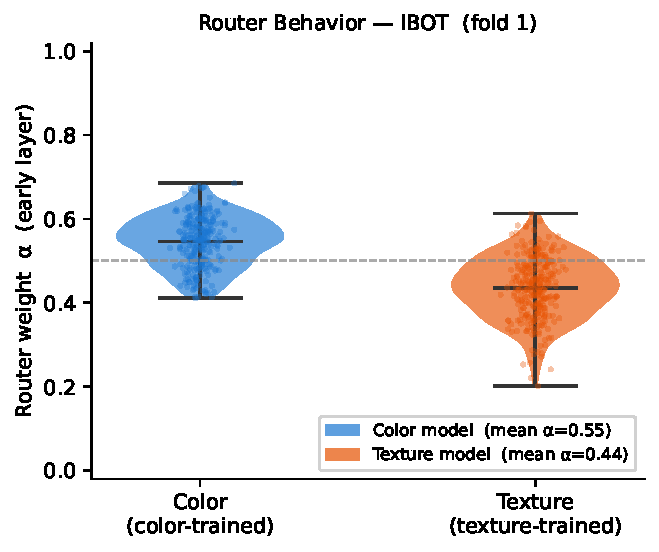
\includegraphics[width=0.46\textwidth]{fig_router_behavior.pdf}}
\caption{Distribui\c{c}\~{a}o dos pesos $\alpha$ do roteador para a
         camada inicial, nos modelos MoE treinados para cor e textura
         (iBOT, fold~1). O modelo de cor atribui maior peso \`{a} camada
         inicial (mediana $\alpha \approx 0,55$), enquanto o de textura
         desloca-se para a camada profunda ($\alpha \approx 0,44$).}
\label{fig_router}
\end{figure}

A exce\c{c}\~{a}o do iBOT textura~($-$2,40~pp sobre Exp.~1) deve-se ao
fato de o Bloco~9 j\'{a} fornecer representa\c{c}\~{o}es excepcionalmente
ricas~(97,20\%); o roteador n\~{a}o melhora o que j\'{a} est\'{a} pr\'{o}ximo
do teto do conjunto.
Para VGG-16 em cor, a assimetria dimensional entre a camada inicial
pequena~(64d) e a profunda~(256d) pode limitar a capacidade do projetor
$h_E$.

Em termos pr\'{a}ticos, o MoE oferece uma representa\c{c}\~{a}o unificada
para sistemas de recupera\c{c}\~{a}o por atributo visual, eliminando a
necessidade de selecionar manualmente a camada mais adequada para cada
tipo de consulta.

Os resultados CBIR fornecem evid\^{e}ncias adicionais de que a fus\~{a}o
adaptativa proposta melhora n\~{a}o apenas o desempenho de classifica\c{c}\~{a}o,
mas tamb\'{e}m a estrutura do espa\c{c}o de embedding.
Na maioria dos backbones, ganhos em acur\'{a}cia s\~{a}o acompanhados de
ganhos consistentes em mAP@10, R@1 e R@5, indicando que imagens
semanticamente relacionadas tornam-se mais agrupadas.
Curiosamente, as melhorias de recupera\c{c}\~{a}o s\~{a}o frequentemente
maiores do que os ganhos correspondentes em acur\'{a}cia, sugerindo que o
MoE aprimora a organiza\c{c}\~{a}o da vizinhan\c{c}a al\'{e}m do que a
acur\'{a}cia de classifica\c{c}\~{a}o isolada captura.
Esse efeito \'{e} especialmente vis\'{i}vel para iBOT no conjunto de cor,
onde o MoE eleva o mAP@10 de 94,93\% para 97,96\%, corrigindo
simultaneamente a severa degrada\c{c}\~{a}o introduzida pela concatena\c{c}\~{a}o
simples.
Em contrapartida, nos casos em que uma camada especializada j\'{a} atinge
desempenho de recupera\c{c}\~{a}o pr\'{o}ximo ao teto --- como o Bloco~9
do iBOT para textura --- o MoE oferece pouco benef\'{i}cio adicional,
indicando que a representa\c{c}\~{a}o subjacente j\'{a} \'{e} altamente
discriminativa.

% -----------------------------------------------------------------------
\section{Conclus\~{o}es}

Este trabalho avaliou a extra\c{c}\~{a}o de caracter\'{i}sticas por
camada em cinco arquiteturas de aprendizado profundo para classifica\c{c}\~{a}o
de cor e textura, e propôs um modelo de fus\~{a}o adaptativa baseado em MoE.
O padr\~{a}o de sensibilidade por camada --- camadas iniciais para cor,
profundas para textura --- generaliza-se de CNNs a Vision Transformers e
SSMs, e a concatena\c{c}\~{a}o simples n\~{a}o \'{e} uma estrat\'{e}gia
eficaz de fus\~{a}o.
O MoE supera ambas as baselines em 5 das 8 configura\c{c}\~{o}es e empata
com a baseline de camada \'{u}nica em mais um caso, atingindo 98,13\%
(VMamba, textura) e 98,13\% (iBOT, cor), e fornece uma representa\c{c}\~{a}o
unificada que se adapta ao conte\'{u}do da imagem sem sele\c{c}\~{a}o
manual de camada.
Trabalhos futuros explorar\~{a}o mais de dois especialistas, aten\c{c}\~{a}o
entre camadas e recupera\c{c}\~{a}o em larga escala.

% -----------------------------------------------------------------------
\section*{Agradecimentos}

Este trabalho foi apoiado pelo Conselho Nacional de Desenvolvimento
Cient\'{i}fico e Tecnol\'{o}gico (CNPq, Brasil).

% -----------------------------------------------------------------------
\begin{thebibliography}{00}

\bibitem{b1}
S. R. Dubey, ``A decade survey of content based image retrieval using deep
learning,'' \emph{IEEE Trans. Circuits Syst. Video Technol.}, vol.~32,
no.~5, pp.~2687--2704, 2021.

\bibitem{b2}
A. Baloian, N. Murrugarra-Llerena, and J. M. Saavedra, ``Scalable visual
attribute extraction through hidden layers of a residual convnet,''
\emph{arXiv preprint arXiv:2104.00161}, 2021.

\bibitem{b3}
J. Deng, W. Dong, R. Socher, L.-J. Li, K. Li, and L. Fei-Fei,
``ImageNet: A large-scale hierarchical image database,'' in
\emph{Proc. IEEE CVPR}, 2009, pp.~248--255.

\bibitem{b4}
K. He, X. Zhang, S. Ren, and J. Sun, ``Deep residual learning for image
recognition,'' in \emph{Proc. IEEE CVPR}, 2016, pp.~770--778.

\bibitem{b7}
K. Simonyan and A. Zisserman, ``Very deep convolutional networks for
large-scale image recognition,'' \emph{arXiv preprint arXiv:1409.1556},
2014.

\bibitem{b8}
M. Moresco, A. D. S. Britto, Y. M. Costa, L. J. Senger, and
A. G. Hochuli, ``Combining multi-layer features for plant species
classification in a Siamese network,'' in \emph{Proc. IEEE SMC}, 2022,
pp.~2446--2451.

\bibitem{b10}
K. Liang, H. Chang, S. Shan, and X. Chen, ``A unified multiplicative
framework for attribute learning,'' in \emph{Proc. IEEE ICCV}, 2015,
pp.~2506--2514.

\bibitem{b11}
C. Gan, T. Yang, and B. Gong, ``Learning attributes equals multi-source
domain generalization,'' in \emph{Proc. IEEE CVPR}, 2016, pp.~87--97.

\bibitem{b12}
S. M. Youssef, ``ICTEDCT-CBIR: Integrating curvelet transform with
enhanced dominant colors extraction and texture analysis for efficient
content-based image retrieval,'' \emph{Comput. Electr. Eng.}, vol.~38,
no.~5, pp.~1358--1376, 2012.

\bibitem{b13}
A. Irtaza, M. A. Jaffar, E. Aleisa, and T. S. Choi, ``Embedding neural
networks for semantic association in content based image retrieval,''
\emph{Multimedia Tools Appl.}, vol.~72, pp.~1911--1931, 2014.

\bibitem{b15}
C. H. Lin, R. T. Chen, and Y. K. Chan, ``A smart content-based image
retrieval system based on color and texture feature,'' \emph{Image Vis.
Comput.}, vol.~27, no.~6, pp.~658--665, 2009.

\bibitem{b16}
A. Gu and T. Dao, ``Mamba: Linear-time sequence modeling with selective
state spaces,'' \emph{arXiv preprint arXiv:2312.00752}, 2023.

\bibitem{b17}
J. Zhou et al., ``iBOT: Image BERT pre-training with online tokenizer,''
\emph{arXiv preprint arXiv:2111.07832}, 2021.

\bibitem{b23}
D. Mukherjee, R. Mondal, P. K. Singh, R. Sarkar, and D. Bhattacharjee,
``EnsembleNet: A hybrid approach for vehicle detection and traffic density
estimation based on Faster R-CNN and YOLO,'' \emph{Neural Comput. Appl.},
vol.~32, no.~15, pp.~14207--14228, 2020.

\bibitem{b24}
J. Yue, Z. Li, L. Liu, and Z. Fu, ``Content-based image retrieval using
color and texture,'' in \emph{Proc. ICIG}, 2011, pp.~833--837.

\bibitem{b25}
E. Prakasa, ``Texture feature extraction by using local binary pattern,''
\emph{INKOM J.}, vol.~1, no.~1, pp.~1--6, 2016.

\bibitem{b26}
J. Long, E. Shelhamer, and T. Darrell, ``Fully convolutional networks for
semantic segmentation,'' in \emph{Proc. IEEE CVPR}, 2015, pp.~3431--3440.

\bibitem{b27}
Y. Guo, Y. Liu, T. Georgiou, and M. S. Lew, ``A review of semantic
segmentation using deep neural networks,'' \emph{Int. J. Multimedia Inf.
Retr.}, vol.~7, no.~2, pp.~87--93, 2018.

\bibitem{b28}
J. de Matos, L. E. S. de Oliveira, A. D. S. Britto Jr., and
A. L. Koerich, ``Large-margin representation learning for texture
classification,'' \emph{Pattern Recognit. Lett.}, vol.~170, pp.~39--47,
2023.

\bibitem{bzeiler}
M. D. Zeiler and R. Fergus, ``Visualizing and understanding convolutional
networks,'' in \emph{Proc. ECCV}, 2014, pp.~818--833.

\bibitem{bkazami}
H. Kazami, N. Touvron, M. Cord, and P. Perez, ``What do vision
transformers learn? A visual exploration,''
\emph{arXiv preprint arXiv:2212.06727}, 2022.

\bibitem{bmoe_orig}
R. A. Jacobs, M. I. Jordan, S. J. Nowlan, and G. E. Hinton,
``Adaptive mixtures of local experts,''
\emph{Neural Computation}, vol.~3, no.~1, pp.~79--87, 1991.

\bibitem{bmoe_cao}
Z. Cao et al., ``Multi-modal gated mixture of local-to-global experts for
dynamic image fusion,'' in \emph{Proc. IEEE/CVF ICCV}, 2023,
pp.~23555--23564.

\end{thebibliography}

\end{document}
